\documentclass[12pt,a4paper]{article}

\usepackage[utf8]{inputenc}
\usepackage[T1]{fontenc}
\usepackage{geometry}
\geometry{margin=2.5cm}
\usepackage{graphicx}
\usepackage{listings}
\usepackage{xcolor}
\usepackage{hyperref}
\usepackage{booktabs}
\usepackage{float}
\usepackage{amsmath}
\usepackage{tikz}
\usetikzlibrary{positioning, arrows.meta, shapes.geometric}

\lstset{
    basicstyle=\ttfamily\small,
    backgroundcolor=\color{gray!10},
    frame=single,
    breaklines=true,
    columns=fullflexible,
    keepspaces=true
}

\begin{document}

\begin{titlepage}
\centering
\vspace*{\fill}
{\LARGE \textbf{Project 3 -- DEX-NFT Pawning Dapp}}\\[0.5cm]
{\large Decentralized Computing and Blockchains}\\[0.3cm]
{2025/2026}\\[1.5cm]

\includegraphics[width=0.65\textwidth]{figures/ciencias_logo_atualizado.png}\\[1.5cm]
Lenny Briclet (66926)\\
Valentin Barner (66958)\\
\today
\vspace*{\fill}
\thispagestyle{empty}
\end{titlepage}
\newpage
\setcounter{page}{1}

\section{Introduction}

This report describes the implementation of a decentralized application (Dapp) that combines a DEX (Decentralized EXchange) marketplace, an NFT marketplace with fixed-price sales and auctions, and two lending mechanisms: one backed by DEX collateral and another backed by NFT collateral with a third-party DEX backer. The project follows the Solidity, Hardhat and ethers.js practices presented during the course. It satisfies the six functionalities listed in the project statement and respects the rule that all financial logic must reside on-chain, while off-chain state is restricted to NFT metadata such as names, descriptions and image URLs.

\section{Architecture}

The system is split between three on-chain smart contracts (Solidity 0.8.28) and two off-chain components, as shown in Figure~\ref{fig:arch}.

\begin{itemize}
    \item \textbf{DexToken} (ERC20) implements the DEX fungible token and the buy/sell operations against ETH at a configurable rate.
    \item \textbf{NftCollection} (ERC721) lets users mint, burn and look up NFTs. It also stores an on-chain value used by the lending logic.
    \item \textbf{PawningHub} is the orchestrator. It coordinates loans, marketplace listings, auctions and the administrator console. After deployment its ownership of DexToken allows the admin to change parameters from a single entry point.
    \item A small \textbf{Express server} on port 3001 stores NFT metadata (name, description, image URL) only. It holds no funds and makes no financial decision.
    \item A static \textbf{web frontend} (HTML + ethers.js v5) connects through MetaMask, calls the three contracts and queries the metadata server.
\end{itemize}

\noindent The Hardhat network (chain ID 31337) is used for local testing and demonstration.

\begin{figure}[H]
\centering
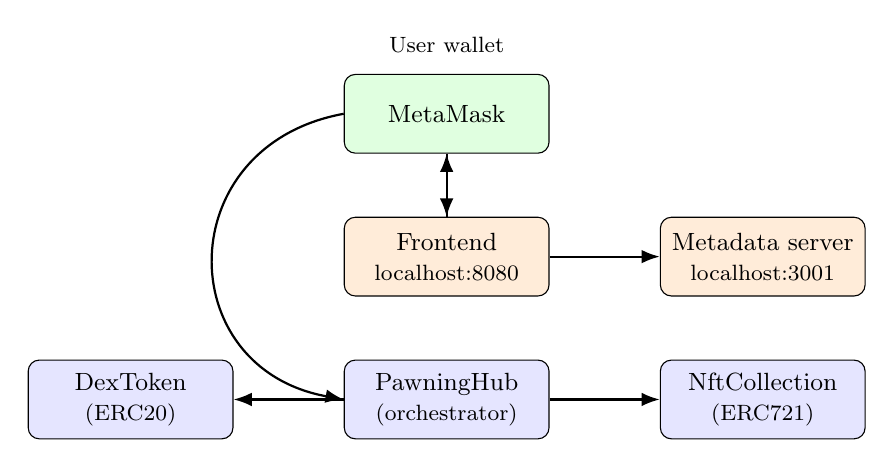
\begin{tikzpicture}[
    node distance=0.8cm and 1.4cm,
    box/.style={rectangle, draw, rounded corners, minimum height=1cm, minimum width=2.6cm, align=center, font=\small},
    chain/.style={box, fill=blue!10},
    off/.style={box, fill=orange!15},
    user/.style={box, fill=green!12},
    arrow/.style={-Latex, thick}
]

\node[user] (mm) {MetaMask};
\node[off, below=of mm] (front) {Frontend\\ \footnotesize localhost:8080};
\node[off, right=of front] (srv) {Metadata server\\ \footnotesize localhost:3001};

\node[chain, below=of front] (hub) {PawningHub\\ \footnotesize (orchestrator)};
\node[chain, left=of hub] (dex) {DexToken\\ \footnotesize (ERC20)};
\node[chain, right=of hub] (nft) {NftCollection\\ \footnotesize (ERC721)};

\draw[arrow] (mm) -- (front);
\draw[arrow] (front) -- (mm);
\draw[arrow] (front) -- (srv);
\draw[arrow] (mm.west) .. controls +(-2.2cm,-0.4cm) and +(-2.2cm,0.4cm) .. (hub.west);
\draw[arrow] (hub) -- (dex);
\draw[arrow] (hub) -- (nft);

\node[above=0.15cm of mm, font=\footnotesize] {User wallet};
\end{tikzpicture}
\caption{System architecture: three on-chain contracts (blue) plus two off-chain components (orange).}
\label{fig:arch}
\end{figure}

\section{Functionalities}

\subsection{DEX Marketplace}
DexToken initialises a fixed pool of DEX held by the contract itself and exposes a swap rate measured in wei per DEX. The \texttt{buyDex()} function sends \texttt{msg.value / dexSwapRate} DEX to the caller and \texttt{sellDex(amount)} performs the reverse. The contract is funded with ETH during deployment so users can withdraw value when selling.

\subsection{Ether Loans with DEX Collateral}
A borrower opens a loan with \texttt{loanDex(dexAmount, duration)}. The hub escrows the collateral, applies a 50\% loan-to-value ratio and transfers ETH to the borrower. The duration is split into payment cycles; each cycle the borrower pays a fixed interest slice through \texttt{makeDexPayment}. A missed cycle triggers \texttt{\_liquidateDexLoan} on the next payment call and the collateral is transferred to the protocol. The borrower can close the loan early using \texttt{terminateDexLoan}, which charges a fixed termination fee in addition to the remaining interest.

\subsection{NFT Marketplace}
NftCollection lets any user mint NFTs through \texttt{mint(uri, valueInWei)} and destroy them with \texttt{burn(tokenId)}. The URI points to the metadata server. Sellers list NFTs for a fixed price using \texttt{listFixed}; buyers pay with either ETH or DEX. The hub performs the conversion using the current swap rate, so a listing priced in one currency can be paid in the other. On every sale the seller receives 95\% of the price and the Dapp owner collects a 5\% protocol fee in the listing currency.

\subsection{NFT Auctions}
\texttt{listAuction} creates a time-bound listing with a minimum price and a maximum wait. Each call to \texttt{bid} must exceed the previous bid; the previous bidder is automatically refunded. After the deadline anyone calls \texttt{finalizeAuction}: the NFT moves to the highest bidder and the winning bid is split between the seller (95\%) and the owner (5\%), in the auction currency. If no bid was placed, the NFT is returned to the seller.

\subsection{NFT-Backed Loans with DEX Backer}
The platform cannot own arbitrary NFTs, so NFT-backed loans rely on a third actor, the \emph{backer}. The borrower calls \texttt{requestNftLoan}; the NFT is escrowed. A backer then calls \texttt{fundNftLoan}, supplying the required DEX, and the hub releases ETH to the borrower (50\% of the NFT's on-chain value). Half of every interest payment is forwarded to the backer through \texttt{makeNftPayment}. On normal closure, the backer recovers the DEX and half of the remaining interest plus half of the termination fee. On default, both the NFT and the DEX backing are transferred to the backer; this is the incentive that makes such loans possible.

\subsection{Administrator Console}
PawningHub exposes \texttt{onlyOwner} setters for the payment cycle, interest percentage, termination fee, maximum loan duration and DEX swap rate, plus withdraw functions for ETH and DEX held by the contract. The frontend shows an Administrator tab only when the connected account equals \texttt{hub.owner()}.

\section{Security and Design Choices}

All money handling lives in the smart contracts. Every external function that moves value uses OpenZeppelin's \texttt{ReentrancyGuard}, \texttt{SafeERC20} wrappers and explicit access control through \texttt{Ownable}. State updates always precede external calls (Checks-Effects-Interactions). Liquidations are deterministic so no off-chain oracle is required. The metadata server only serves and persists JSON; an outage or corruption there never affects on-chain balances. The frontend uses MetaMask for signing and verifies the network (chain ID 31337) before any transaction, recreating the provider when the chain changes to avoid network-mismatch errors. Setup and execution instructions are provided in the project \texttt{README.md}; the contract logic is also covered by 28 Hardhat tests that all pass.

\section{Use of AI}
The projects setup and core structure was done with the Help of Github Copilot Agent. 
This includes:
\begin{itemize}
    \item npm and harthat setup
    \item initial version of frontend, server and smart contract code.
\end{itemize}
Refining, bug fixing and testing has been done manually and with the help of AI.
\end{document}
